\chapter{The Law of Large Numbers}
\label{ch:lln}

\begin{chaptergoals}
\begin{itemize}[nosep]
\item Why limits of random variables need different tools than limits of numbers.
\item The sample mean on two scales: collapsing on $\mu$ (this chapter) and, magnified by $\sqrt{n}$, settling into a Gaussian (the next).
\item Convergence in probability, the mode of convergence that says an estimator gets close to what it estimates.
\item The Weak Law of Large Numbers, with Chebyshev's inequality as the proof.
\end{itemize}
The running example is the kiss experiment of \cref{ch:kiss}: $n = 124$ couples, $80$ of whom turned right, so $\hat{p} = \bar{R}_n = 0.645$.

\Cref{ch:models} fixed the object inference happens in; this part supplies the three facts about averages that Part III stands on.

\textbf{The next three chapters.}
The rest of the book rests on three limit facts about averages: the Law of Large Numbers (averages settle on their expectations, this chapter), the Central Limit Theorem (the error of an average is Gaussian on the $1/\sqrt{n}$ scale, \cref{ch:clt}), and the rules for transforming limits and plugging in estimates (continuous mapping, Slutsky, the delta method, \cref{ch:limit-tools}).
Those three chapters are the minimal path.
Two more modes of convergence, almost sure and in mean, complete the standard hierarchy; that material is in \cref{app:modes} because nothing later is proved with it; where a later chapter mentions almost sure convergence, the in-probability version is the one in use.
Read it once for orientation and don't spend time mastering it.
\end{chaptergoals}

\begin{intuition}[what `asymptotic' means]
An asymptotic result is a license to replace an unknown sampling distribution by its limiting distribution, usually a Gaussian, with an error the theorem does not tell you.
That is all `asymptotic' ever means in this book.
The definitions below are about infinite sequences, while every application is about one fixed sample size, usually $n = 124$; the theorems say $n \to \infty$ and they get applied at $n = 64$ without further comment.
The gap is real, and \cref{sec:conv-what-limits-buy} in the next chapter says what the alternatives are and why statistical practice accepts the trade.
When a later chapter says `by the CLT' or `asymptotically normal', read it as: for the $n$ at hand, treat this as Gaussian and carry on.
\end{intuition}

\section{Why limits of random variables need new tools}
\label{sec:conv-why}

\Cref{ch:kiss} asked whether $\hat{p}$ is close to $p$ once $n$ is large.
That is a question about a limit, and limits of random variables need their own definition.
In calculus you say that a sequence of real numbers $x_n$ converges to a limit $x$ if, for any $\epsilon > 0$, $\abs{x_n - x} < \epsilon$ for all large $n$ \toolkit{sec:math-limits}.
Convergence is more subtle in probability.
Returning to calculus, suppose that $x_n = x$ for all $n$.
Then, trivially, $\ds \lim_{n \to \infty} x_n = x$.

Consider a probabilistic version of this example.
Suppose that $X_1, X_2, \ldots$ is a sequence of i.i.d.\ r.v.s such that $X_i \iid \Gauss(0,1)$.
Since these all have the same distribution, you might think $X_n$ `converges' to $X \sim \Gauss(0,1)$.
But this can't be right: $X_n - X \sim \Gauss(0, 2)$ for every $n$, so $\Pr(\abs{X_n - X} < \epsilon)$ is the same small number for every $n$ and never improves. (In fact $\Pr(X_n = X) = 0$ for all $n$, since two independent continuous r.v.s are equal with probability zero.\footnote{Why is this true? Let $Y_1$ and $Y_2$ be continuous r.v.s with joint density $f_{Y_1, Y_2}$. Then
\[
\Pr(Y_1 = Y_2) = \iint_D f_{Y_1, Y_2}(y_1, y_2) \, \mathrm{d}y_1 \, \mathrm{d}y_2, \qquad D = \{(y_1,y_2) \in \real^2: y_1 = y_2 \}.
\]
The set $D$ is a line living in two dimensions and hence has no area: you're integrating a bounded function over a region of zero area, so the integral is $0$.
This is the two-dimensional version of the fact that the `area' under a density at a single point is zero.})
This suggests limiting processes involving probabilities require different tools than those limiting processes from calculus.

The central ideas in this chapter and the next are the two most famous results in all of probability theory: the Law(s) of Large Numbers and the Central Limit Theorem.
An understanding of why these results are valid requires an understanding of limiting processes that involve r.v.s.
These limits are conceptually more general than the limits of undergraduate calculus since, as limits of r.v.s, these limits are not limits of numbers but limits of \textit{functions}.

So what is meant by `convergence of random variables'?
And what is a sequence of r.v.s?
Recall that, by definition, an r.v.\ is a mapping from a sample space, $S$, to the real number line \toolkit{sec:math-rv}.
Suppose, to fix ideas, that the outcomes can be listed (a continuous r.v.\ needs a richer sample space, but the picture is the same), so you can write:
\[
S = \{ s_1, \ldots, s_k \}.
\]

This means an r.v.\ $X$ defined on $S$ can be written as:
\[
X(s_i) = x_i, \text{ for } i = 1,\ldots,k.
\]

When you have a sequence of r.v.s it's useful to keep in mind that there's always an underlying sample space.
In particular, each $X_n$ is a function from $S$ to $\real$:
\[
X_n(s_i) = x_{n,i}, \text{ for } i = 1,\ldots,k.
\]

So a sequence of r.v.s is a sequence of functions $X_n: S \to \real$.
Pick an outcome $s_i$ and you get an ordinary sequence of numbers $x_{1,i}, x_{2,i}, x_{3,i}, \ldots$, one such sequence for every outcome.
A \textit{realization} of the sequence is what you see when the experiment is run once and the outcome happens to be $s_i$.

\begin{figure}[htbp]
\centering
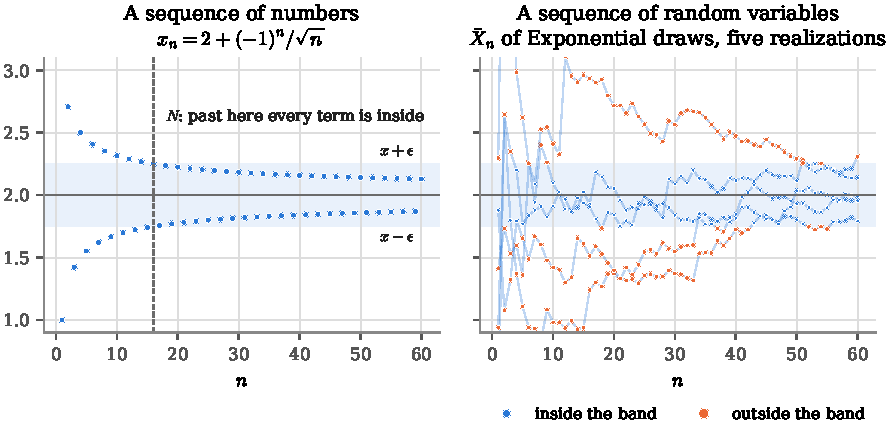
\includegraphics[width=\textwidth]{fig_sequence_vs_random}
\caption{Left: a sequence of numbers converging to $2$. For the band of half-width $\epsilon$ there is an index $N$ past which every term is inside. Right: five realizations of the running sample mean $\bar{X}_n$ of Exponential draws with mean $2$, one path per outcome of the experiment. Each path eventually settles inside the band, but at a different index, and no $N$ works for every path: some realization will leave the band after any $N$ you name. The modes of convergence are different ways of saying `the orange points become rare.'}
\label{fig:seqrand}
\end{figure}

This chapter and the next examine the two modes of convergence this book works with; \cref{app:modes} has the full set.
Why are there different modes of convergence?
Remember that to say a sequence $(X_i)_{i=1}^{\infty}$ converges to $X$ means that the $X_i$'s are getting `closer and closer' to $X$.
Different modes of convergence relate to different ways of defining what `closer' means.
\Cref{fig:seqrand} shows the difficulty: for a sequence of numbers there is a single index $N$ past which every term is within $\epsilon$ of the limit, while for a sequence of r.v.s the index that works depends on the outcome of the experiment and may not exist for some outcomes.

Two of the modes, convergence almost surely and convergence in probability, compare the \textit{values} of $X_n$ and $X$ outcome by outcome, so $X_n$ and $X$ must live on the same sample space.
The third, convergence in distribution, compares the CDFs of $X_n$ and $X$ and never looks at values at all; $X_n$ and $X$ can be defined on entirely different probability spaces.
But as r.v.s have CDFs, the difference between sequences of r.v.s and sequences of CDFs isn't as significant as you might expect.

So it's important to emphasize here that the `things' converging are r.v.s, or their CDFs, and that they converge to an r.v., or a CDF.\footnote{Just because a sequence of r.v.s converges to an r.v.\ doesn't mean the limiting r.v.\ has an interesting distribution or what you normally think of as a `distribution'.
In fact, one mode of convergence explained below (convergence in probability), is almost entirely concerned with the convergence of sequences of r.v.s to a constant or `degenerate' r.v.}

\section{A first look: the sample mean on two scales}
\label{sec:conv-two-scales}

To motivate the notion of convergence of r.v.s, consider the following example.
Suppose that $\Xton$ are i.i.d.\ r.v.s with mean $\mu$ and variance $\sigma^2$ and define the (theoretical, non-realized) sample mean:
\[
\bar{X}_n = \frac{1}{n} \sum_{i=1}^n X_i.
\]

First, consider the behavior of the distribution of $\bar{X}_n$ when $n$ is large.
It seems reasonable that $\bar{X}_n$ will be close to $\mu$ if $n$ is sufficiently large;
that is, the r.v.\ $\bar{X}_n - \mu$ should have a distribution that, for large $n$, is concentrated around 0 or, more precisely:
\[
\Pr(\abs{\bar{X}_n - \mu} \leq \epsilon) \approx 1,
\]

for any small positive number $\epsilon$.
This type of limiting process, and more specifically, that as $n$ increases without limit the probability equals 1, is an example of \textit{convergence in probability}, and also illustrates a convergence process to a constant (here, $\mu$), as discussed in the previous footnote.

Moreover because $\var( \bar{X}_n ) = \sigma^2/n$,\footnote{That $\var( \bar{X}_n ) = \sigma^2/n$ follows from the properties of the variance and the independence of the $X_i$.
Specifically:
\[
\var(\bar{X}_n) = \frac{1}{n^2} \var(X_1 + \cdots + X_n) = \frac{n \sigma^2}{n^2} = \frac{\sigma^2}{n}.
\]} it follows that $\var( \bar{X}_n ) \to 0$ as $n \to \infty$.
Because the variance of $\bar{X}_n$ eventually vanishes as $n$ increases, the limit tells you nothing about the \textit{shape} of the distribution of $\bar{X}_n$: every density in the left panel of \cref{fig:twoviews} is on its way to becoming a spike at $\mu$.

It's possible though to look at the difference between $\bar{X}_n$ and $\mu$ on a `magnified' scale.
To that end, multiply the difference $\bar{X}_n - \mu$ by $\sqrt{n}$, which makes the mean and variance of the resulting r.v.\ constant.
Specifically, define the r.v.\ $Y_n$ by:
\[
Y_n = \sqrt{n}(\bar{X}_n - \mu),
\]

and note that:
\[
\E[Y_n] = \E[\sqrt{n}(\bar{X}_n - \mu)] = \sqrt{n} (\E[\bar{X}_n] - \mu) = \sqrt{n} (\mu - \mu) = 0,
\]

and
\[
\var(Y_n) = \var(\sqrt{n}(\bar{X}_n - \mu)) = n \var(\bar{X}_n - \mu) = n \var(\bar{X}_n) = \sigma^2.
\]

\begin{intuition}[what's special about $\sqrt{n}$?]
Why does multiplying by $\sqrt{n}$, and not by $n$ or by $\log n$, yield a constant mean and variance?
\begin{itemize}[nosep]
\item \textbf{The mean:} Multiplying $\bar{X}_n - \mu$ by anything doesn't impact its expected value because $\bar{X}_n$ is an unbiased estimator of $\mu$, so the expected value of the difference is $0$ to begin with.
\item \textbf{The variance:} As $n$ increases, $\var(\bar{X}_n) = \sigma^2/n$ decreases.
When you multiply an r.v.\ by $\sqrt{n}$ the variance is scaled by a factor of $n$, which exactly cancels the division by $n$.
Multiplying by $n$ instead would scale the variance by $n^2$ and the result would blow up; multiplying by $\log n$ would not be enough and the result would still collapse to a spike.
\end{itemize}
The standard deviation of $\bar{X}_n$ is $\sigma/\sqrt{n}$, so $\sqrt{n}$ is the magnification that holds the spread fixed.
\end{intuition}

\begin{figure}[htbp]
\centering
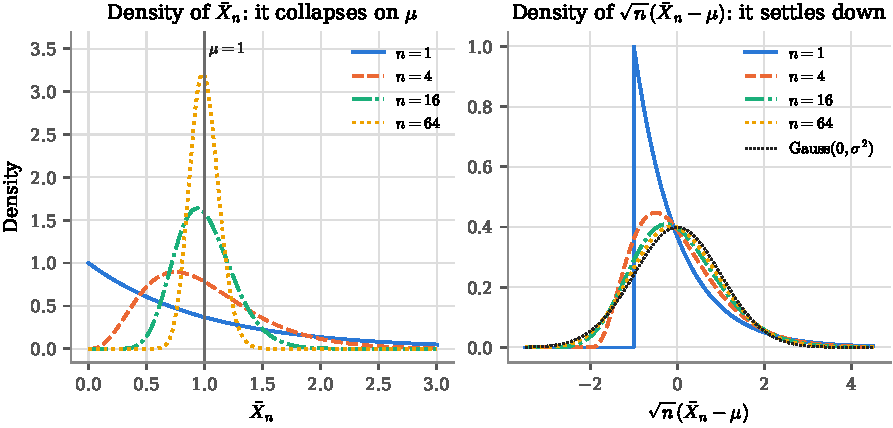
\includegraphics[width=\textwidth]{fig_lln_clt_two_views}
\caption{The same sample mean of $\Expo(1)$ draws on two scales. Left: the density of $\bar{X}_n$ collapses onto $\mu = 1$ as $n$ grows (this is the Law of Large Numbers). Right: after the $\sqrt{n}$ magnification the density of $\sqrt{n}(\bar{X}_n - \mu)$ keeps a fixed spread and its shape settles down to a Gaussian (this is the Central Limit Theorem). At $n = 1$ the magnified density is the skewed exponential itself, shifted; by $n = 64$ it is hard to tell from $\Gauss(0, \sigma^2)$.}
\label{fig:twoviews}
\end{figure}

You can now consider the behavior of the CDF of $Y_n$ as $n$ increases.
If this sequence of CDFs has a limit, then you can use the limiting CDF to approximate the CDF of $Y_n$ (and hence of $\bar{X}_n$).

For example, suppose you have that:
\[
\Pr(Y_n \leq y) = \Pr( \sqrt{n}(\bar{X}_n - \mu) \leq y) \approx F_0(y).
\]

Then, to say something about the CDF of $\bar{X}_n$, subtract $\mu$ from $\bar{X}_n$ and multiply this difference by $\sqrt{n}$, to get:
\[
\Pr(\bar{X}_n \leq x) = \Pr( \sqrt{n}(\bar{X}_n - \mu)  \leq \sqrt{n}(x - \mu)) \approx F_0(\sqrt{n}(x - \mu)),
\]

provided $n$ is sufficiently large to make the approximation valid.
This type of limiting process is an example of \textit{convergence in distribution}, which is the subject of \cref{ch:clt}.

What if instead of transforming $\bar{X}_n$ into $Y_n$, you `standardized' it by dividing $Y_n$ by $\sigma$.
That is, define the r.v.\ $Z_n$ by:
\[
Z_n = \sqrt{n} \left( \frac{\bar{X}_n - \mu}{\sigma} \right).
\]

Now, calculate $\E[Z_n]$ and $\var(Z_n)$:
\[
\E[Z_n] = \E \left[ \sqrt{n} \left( \frac{\bar{X}_n - \mu}{\sigma} \right) \right] = \frac{\sqrt{n}}{\sigma} (\E[\bar{X}_n] - \mu) = \frac{\sqrt{n}}{\sigma} (\mu - \mu) = 0.
\]

Thus, $\E[Y_n] = \E[Z_n] = 0$.
But observe that $\var(Z_n) \neq \var(Y_n) = \sigma^2$:
\begin{align*}
\var(Z_n) &= \var \left( \sqrt{n} \left( \frac{\bar{X}_n - \mu}{\sigma} \right) \right) \\
 &= \frac{n}{\sigma^2} \var \left( \bar{X}_n \right) \\
 &= \frac{n}{\sigma^2} \var \left( \frac{1}{n} \sum_{i=1}^n X_i \right)  \\
 &= \frac{1}{n \sigma^2} \var \left( \sum_{i=1}^n X_i \right) \\
 &= \frac{n \sigma^2}{n \sigma^2} \\
 &= 1.
\end{align*}

Thus, despite the extra scaling factor, $\sqrt{n}$, the r.v.\ $Z_n$ has a `standard' look to it: Its mean is 0 and its variance is 1.
It may not come as a surprise that $Z_n$ converges in distribution to a standard Gaussian distribution.

\begin{bridge}[the standard error]
An introductory course states, usually without proof, that the sampling distribution of the sample mean has mean $\mu$, has standard deviation $\sigma/\sqrt{n}$ (the \textit{standard error} of the mean), and is approximately normal when $n$ is large.
The two panels of \cref{fig:twoviews} are the two halves of that statement.
The standard error shrinking to zero is what drives the Law of Large Numbers.
The shape becoming normal is the Central Limit Theorem.
Dividing $\bar{X}_n - \mu$ by the standard error $\sigma/\sqrt{n}$ is exactly the standardization that produces $Z_n$:
\[
Z_n = \frac{\bar{X}_n - \mu}{\sigma/\sqrt{n}} = \sqrt{n} \left( \frac{\bar{X}_n - \mu}{\sigma} \right).
\]
This chapter proves the first half; \cref{ch:clt} makes `approximately normal when $n$ is large' into a theorem and says what `large' buys you.
\end{bridge}

\section{Convergence in probability}
\label{sec:conv-prob}

Convergence in probability considers the distance between a sequence of r.v.s $X_n$ and some number $x$ being at least as large as some arbitrary $\epsilon > 0$.
That is, in formal terms you're concerned with whether the probability of $\abs{X_n - x} \geq \epsilon$ converges to 0.

A first step in such problems, and limit problems generally, is to grasp the meaning of $\abs{X_n - x} \geq \epsilon$.
An absolute value can be thought of as the distance from 0.
So $\abs{X_n - x}$ is the distance of the number $X_n - x$ from 0, and the event $\abs{X_n - x} \geq \epsilon$ says that this distance is at least $\epsilon$, which happens either when $X_n - x \geq \epsilon$ or when $X_n - x \leq - \epsilon$.
A visualization along the real line is instructive.

\begin{center}
\begin{tikzpicture}[x=1cm, y=1cm]
  \draw[-{Latex[length=2mm]}, gray] (-4.6,0) -- (4.6,0);
  \draw[very thick, boxorange, -{Latex[length=2mm]}] (1.6,0) -- (4.3,0);
  \draw[very thick, boxorange, -{Latex[length=2mm]}] (-1.6,0) -- (-4.3,0);
  \draw[very thick, boxblue] (-1.6,0) -- (1.6,0);
  \fill[boxorange] (1.6,0) circle (2pt);
  \fill[boxorange] (-1.6,0) circle (2pt);
  \draw (0,0.1) -- (0,-0.1);
  \node[below] at (0,-0.1) {$0$};
  \node[below] at (1.6,-0.1) {$\epsilon$};
  \node[below] at (-1.6,-0.1) {$-\epsilon$};
  \node[above, font=\small] at (3.0,0.1) {$X_n - x \geq \epsilon$};
  \node[above, font=\small] at (-3.0,0.1) {$X_n - x \leq -\epsilon$};
  \node[above, font=\small, boxblue!70!black] at (0,0.1) {$\abs{X_n - x} < \epsilon$};
\end{tikzpicture}
\end{center}

If a sequence of r.v.s converges in probability to a number, say, 0, then you say the sequence converges to the zero \textit{random variable} (not the number 0).
Now for the definition.

\begin{definition}[Convergence in probability]
\label{def:convp}
A sequence of r.v.s, $(X_n)_{n \geq 1}$, \textbf{converges in probability} to an r.v.\ $X$ if, for every $\epsilon > 0$:
\[
\lim_{n \to \infty} \Pr(\abs{X_n - X} \geq \epsilon) = 0, \, \text{ or equivalently } \, \lim_{n \to \infty} \Pr(\abs{X_n - X} < \epsilon) = 1.
\]
If $(X_n)_{n \geq 1}$ converges in probability to some r.v.\ $X$, then this is denoted by $X_n \convp X$.
\end{definition}

\begin{inwords}
\textbf{In words.} Read the definition from the inside out. Fix a tolerance $\epsilon$. For each $n$, $\Pr(\abs{X_n - X} \geq \epsilon)$ is a number, the probability mass that $X_n$ puts outside the $\epsilon$-band around $X$. The definition says this sequence of \textit{numbers} goes to $0$ in the ordinary calculus sense \toolkit{sec:math-limits}, and that it must do so for every tolerance, however small. Nothing is said about any single outcome; everything is said about probabilities.
\par\smallskip
\textbf{For the kiss data.} $\bar{R}_n \convp p$ means: pick any tolerance, say $0.01$; the probability that the sample proportion turning right misses $p$ by more than $0.01$ can be made as small as you like by observing enough couples. It does not say how many couples; \cref{sec:wlln} and \cref{ch:clt} do.
\end{inwords}
\Cref{fig:convpband} shows the picture for the sample mean, where $X$ is the constant $\mu$.

\begin{figure}[htbp]
\centering
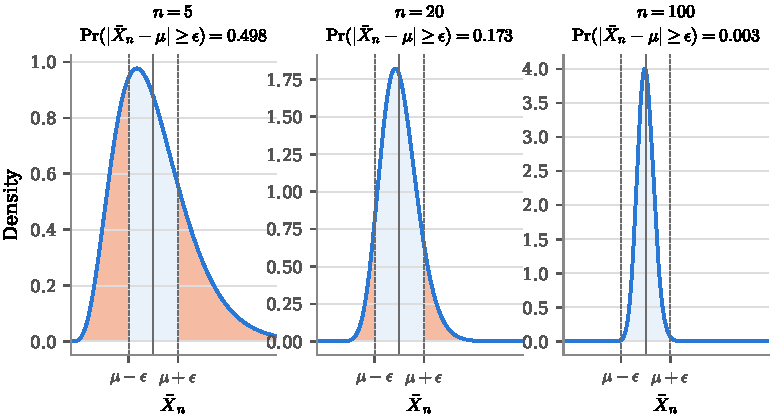
\includegraphics[width=\textwidth]{fig_conv_prob_band}
\caption{Convergence in probability as a picture. The density of $\bar{X}_n$ for $\Expo(1)$ draws at three sample sizes, with the band $[\mu - \epsilon, \mu + \epsilon]$ for $\epsilon = 0.3$. The shaded orange mass is $\Pr(\abs{\bar{X}_n - \mu} \geq \epsilon)$; it goes from about one half at $n = 5$ to essentially zero at $n = 100$. Shrink $\epsilon$ and the same thing happens, only it takes a larger $n$.}
\label{fig:convpband}
\end{figure}

Though convergence in probability is defined as a sequence of r.v.s converging to an r.v., in statistical applications the limit is almost always a constant: the sample mean converges to $\mu$, an estimator converges to the parameter it estimates.
There's a reason the interesting limits are constants.
If the r.v.s in the sequence are independent and the sequence converges in probability, then the limiting r.v.\ must be a constant.\footnote{A sketch, not a proof, and not needed later: the limit of a sequence can't depend on any finite number of its terms (throw away the first million terms and the limit is unchanged). If the terms are independent, the limit is therefore independent of every one of them, hence independent of everything that's random in the experiment, hence independent of itself. An r.v.\ independent of itself satisfies $\var(X) = \cov(X, X) = 0$, so it's a constant. The precise statement is Kolmogorov's zero-one law.}
The sample mean $\bar{X}_n$ isn't a sequence of independent r.v.s (each $\bar{X}_n$ shares $X_1$ with all the others), so this fact doesn't apply to it directly, but the conclusion is the same: the randomness averages out.

\subsection{Example: the minimum of uniforms}

\begin{example}
\label{ex:min-unif}
Let $X_1, X_2, \ldots \iid \text{Unif}([0,1])$ and define the minimum of the first $n$ by $\ds X_{(1)} = \min_{i=1,\ldots,n} X_i$.
Then:
\[
X_{(1)} \convp 0.
\]
\end{example}

\coreproof{Write the event $\abs{X_{(1)} - 0} \geq \epsilon$ as an event about the whole sample, use independence to turn its probability into a product of $n$ equal factors, and let $n \to \infty$. This is the template for every direct convergence proof that follows.}
\begin{proof}
\leavevmode % Puts first item on next line
\begin{itemize}

\item Let $\epsilon > 0$.
Write the claim using the definition of convergence in probability: you need $\Pr(\abs{X_{(1)} - 0} \geq \epsilon) \to 0$.

\item Now, you'll simplify the expression in such a way as to eventually take the limit of the expression as $n \to \infty$.

\item To that end, observe that:
\begin{align*}
\Pr(\abs{X_{(1)} - 0} \geq \epsilon) &= \Pr(\abs{X_{(1)}} \geq \epsilon) \\
								&= \Pr(X_{(1)} \geq \epsilon) \\
								&= \Pr(X_1 \geq \epsilon, X_2 \geq \epsilon, \ldots, X_n \geq \epsilon) \\
								&= \Pr(X_1 \geq \epsilon) \Pr(X_2 \geq \epsilon) \cdots \Pr(X_n \geq \epsilon) \\
								&= \Pr(X_1 \geq \epsilon)^n.
\end{align*}

The movement from the second to the third equality holds because, as $X_{(1)}$ is the minimum of the $X_i$'s, the minimum is at least $\epsilon$ exactly when every $X_i$ is at least $\epsilon$: the single event is equivalent to the joint event.
The fourth equality results since the $X_i$'s are independent, and the fifth since they're identically distributed.

\item You know that $X_1 \sim \text{Unif}([0,1])$.
Therefore, $f_{{X}_1}(x) = 1$ for all values in $X_1$'s support.

\item This implies that $\ds \Pr(X_1 \geq \epsilon) = \int_{\epsilon}^1 1 \dx = 1 - \epsilon$, and further that:
\[
\Pr(X_1 \geq \epsilon)^n = (1 - \epsilon)^n.
\]

Also, note that $1 - \epsilon$ is some number between 0 and 1 (for $\epsilon \geq 1$ the probability is already $0$, so there's nothing to prove).

\item Now you're ready to take the limit of this probability and confirm the statement:
\[
\lim_{n \to \infty} \Pr(\abs{X_{(1)} - 0} \geq \epsilon) = \lim_{n \to \infty} (1 - \epsilon)^n = 0,
\]

and hence $X_{(1)} \convp 0$, as desired.
\end{itemize}
\end{proof}

\begin{figure}[htbp]
\centering
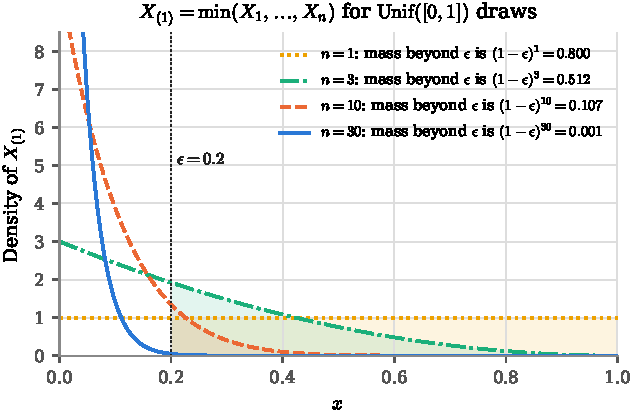
\includegraphics[width=0.8\textwidth]{fig_min_uniform}
\caption{\Cref{ex:min-unif} as a picture. The density of $X_{(1)} = \min(X_1, \ldots, X_n)$ is $n(1-x)^{n-1}$ on $[0,1]$. As $n$ grows the mass piles up against $0$, and the mass beyond $\epsilon$, which is the $(1-\epsilon)^n$ of the proof, goes to zero. The proof computes the shaded tail; the picture shows why it has to shrink. (The $n = 10$ and $n = 30$ curves are cut off at the top; their peaks are at $10$ and $30$.)}
\label{fig:minunif}
\end{figure}

The proof is the template for every direct proof of convergence in probability: write the event $\abs{X_n - X} \geq \epsilon$, rewrite it as an event about the original sample, use independence to turn a joint probability into a product, and take the limit.

\subsection{A workhorse: shrinking variance}

Most of the time you won't compute $\Pr(\abs{X_n - x} \geq \epsilon)$ directly.
You'll use the following criterion, which only needs a mean and a variance.

\begin{proposition}[Shrinking-variance criterion]
\label{prop:shrinking-variance}
Let $(T_n)_{n \geq 1}$ be a sequence of r.v.s with $\E[T_n] \to \mu$ and $\var(T_n) \to 0$.
Then $T_n \convp \mu$.
\end{proposition}

\coreproof{Chebyshev's inequality bounds the probability of a large deviation by a variance; a variance going to $0$ drags the probability with it. The triangle inequality handles the mean not being exactly $\mu$ \toolkit{sec:math-inequalities}.}
\begin{proof}
The argument is Chebyshev's inequality.
Recall its two ingredients.
\textit{Markov's inequality:} if $Y \geq 0$ then $\Pr(Y \geq a) \leq \E[Y]/a$ for every $a > 0$.
\textit{Chebyshev's inequality:} applying Markov's inequality to $Y = (T - \E[T])^2$ with $a = \epsilon^2$ gives, for any r.v.\ $T$ with finite variance,
\[
\Pr(\abs{T - \E[T]} \geq \epsilon) \leq \frac{\var(T)}{\epsilon^2}.
\]
Now fix $\epsilon > 0$.
For $n$ large enough that $\abs{\E[T_n] - \mu} < \epsilon/2$, the event $\abs{T_n - \mu} \geq \epsilon$ forces $\abs{T_n - \E[T_n]} \geq \epsilon/2$ (triangle inequality), so
\[
\Pr(\abs{T_n - \mu} \geq \epsilon) \leq \Pr(\abs{T_n - \E[T_n]} \geq \epsilon/2) \leq \frac{4 \var(T_n)}{\epsilon^2} \to 0. \qedhere
\]
\end{proof}

\begin{example}
\label{ex:bern-1-over-n}
Let $X_n \sim \Bern(1/n)$, so $X_n$ is $1$ with probability $1/n$ and $0$ otherwise.
For $0 < \epsilon < 1$, $\Pr(\abs{X_n - 0} \geq \epsilon) = \Pr(X_n = 1) = 1/n \to 0$, so $X_n \convp 0$.
Alternatively, $\E[X_n] = 1/n \to 0$ and $\var(X_n) = \frac{1}{n}(1 - \frac{1}{n}) \to 0$, and \cref{prop:shrinking-variance} gives the same conclusion.
\end{example}

\section{The Weak Law of Large Numbers (WLLN)}
\label{sec:wlln}

Frequently, statisticians are concerned with situations in which the limiting r.v.\ is a constant and the r.v.s in the sequence are sample means.
The most famous result along these lines is the Weak Law of Large Numbers (WLLN), which is stated here but explained and proved below.

\begin{theorem}[Weak Law of Large Numbers]
\label{thm:wlln}
Let $X_1, X_2, \ldots$ be i.i.d.\ r.v.s with $\E[X_i] = \mu$ and $\var(X_i) = \sigma^2 < \infty$, and let $\bar{X}_n$ be the sample mean.
Then, for every $\epsilon > 0$:
\[
\lim_{n \to \infty} \Pr(\abs{\bar{X}_n - \mu} < \epsilon) = 1.
\]
That is, $\bar{X}_n \convp \mu$.
\end{theorem}

Let's motivate this all-important result.
Suppose you have some probability distribution with a certain mean, $\mu$, and variance, $\sigma^2$, which is assumed finite.
Then you draw $n$ independent r.v.s, $\Xton$, from the distribution so that the $X_i$'s are independent and identically distributed (i.i.d.\ r.v.s).
At this point, make sure you understand that each $X_i$ is an exact copy of the parent r.v.\ you are `drawing' these r.v.s from.
Also, make sure to keep in mind that you're `drawing' r.v.s and not values of r.v.s (i.e., numbers).
You can think of this as carrying out a long experiment during which these r.v.s are drawn.
Once you've drawn all of these r.v.s, you calculate their average that yields the \textbf{(theoretical) sample mean}, $\bar{X}_n$:
\[
\bar{X}_n = \frac{X_1 + \cdots + X_n}{n}.
\]

\textbf{Question:} Why `theoretical' sample mean?

\textbf{Answer:} In order to avoid confusion with the descriptive statistic that also goes by `sample mean', $\bar{X}_n$ is the theoretical sample mean because \textit{it's a random variable}, not a number.
The sample here, $\Xton$, is a sample of $n$ r.v.s, each of which has the same distribution.
If the values of the $X_i$'s are realized, then the descriptive sample mean, the realized value, is easily calculated as:
\[
\bar{x}_n = \frac{x_1 + \cdots + x_n}{n},
\]

where the $x_i$'s are the realized values of the $X_i$'s.
This explanation is given in the hopes that when you see $\bar{X}_n$ your mind doesn't go to the number $\bar{x}_n$.
In the kiss experiment, $\bar{R}_n$ is the r.v.\ `proportion turning right in a sample of $n$ couples' and $\bar{r}_n = 80/124 = 0.645$ is the number the one sample happened to produce.

Notice that $\bar{X}_n$ is itself an r.v.\ because it's a function of r.v.s.
The sample mean isn't the true mean, $\mu$, of the parent distribution; that is, $\bar{X}_n \neq \mu$, although as demonstrated below $\E[\bar{X}_n] = \mu$.
But, $\mu = \E[X_i]$ for all $i$ and is a number (not an r.v.).
This is how it should be since the distribution of every $X_i$ is an exact copy of $X$'s distribution.
As such, the mean of $X$ must equal the mean of the $X_i$'s.
The sample mean is the simplest and most natural way for trying to estimate the true mean, and the Weak Law of Large Numbers (WLLN) offers support to this notion.

Before explaining in more detail the WLLN consider some properties of the sample mean, $\bar{X}_n$.
By linearity, its expectation is:
\[
\E[\bar{X}_n] = \E\left[\frac{X_1 + \cdots + X_n}{n} \right] = \frac{n \mu}{n} = \mu.
\]

The expectation $\E[\bar{X}_n]$ involves two different kinds of averaging, and it's worth separating them.
The sample mean, $\bar{X}_n$, averages over the $n$ draws of one experiment.
The expectation, $\E[\bar{X}_n]$, averages over \textit{all} possible outcomes of that experiment, weighted by their probabilities, which is a theoretical average because you never observe all possible outcomes.
The statement $\E[\bar{X}_n] = \mu$ says that the second kind of average of the first kind of average lands on the true mean.
\Cref{fig:twoaverages} draws the two directions.

\begin{figure}[htbp]
\centering
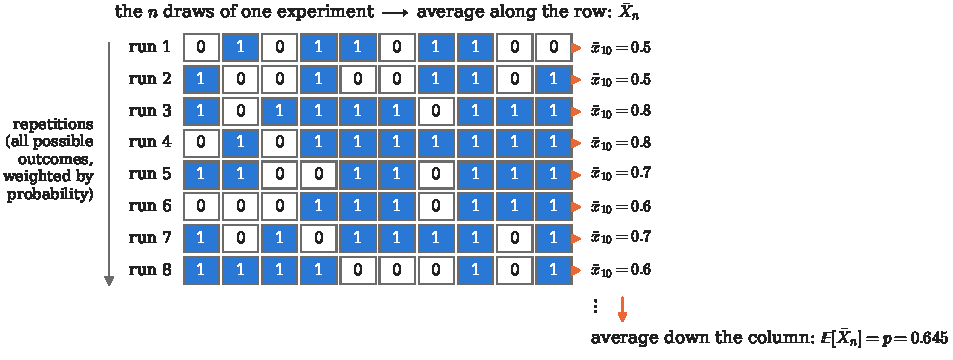
\includegraphics[width=\textwidth]{fig_two_averages}
\caption{Two kinds of averaging. Each row is one run of the experiment, here $n = 10$ Bernoulli draws with $p = 0.645$; averaging along the row gives that run's sample mean, a different number each time. The expectation averages down the column, over every possible run weighted by its probability (only eight runs are shown; the expectation uses all $2^{10}$ of them). The first average is a random variable; the second is the number $p$.}
\label{fig:twoaverages}
\end{figure}

Now, consider the variance of $\bar{X}_n$:
\[
\var(\bar{X}_n) = \frac{\var(X_1 + \cdots + X_n)}{n^2} = \frac{n \sigma^2}{n^2} = \frac{\sigma^2}{n}.
\]

This follows since the $X_i$'s are independent so that the variance of the sum is the sum of the individual variances.

\begin{intuition}[why the variance of the sample mean is scaled by $1/n$]
Averaging $n$ independent draws cancels noise.
Think of each $X_i$ as $\mu + U_i$ where the $U_i$ are independent, mean-zero errors.
Then $\bar{X}_n = \mu + \bar{U}_n$, and the errors in $\bar{U}_n$ have no reason to line up: some are positive, some negative, and summing $n$ of them produces a total whose typical size grows like $\sqrt{n}$, not like $n$ (variances add, so standard deviations add in quadrature).
Dividing by $n$ then leaves a typical error of size $\sigma \sqrt{n}/n = \sigma/\sqrt{n}$.
That's why $\var(\bar{X}_n) = \sigma^2/n$ and why doubling the precision costs four times the data.
\Cref{fig:whyrootn} is that claim drawn: the sum of $n$ cancelling errors reaches about $\sqrt{n}$, not $n$.
\end{intuition}

\begin{figure}[htbp]
\centering
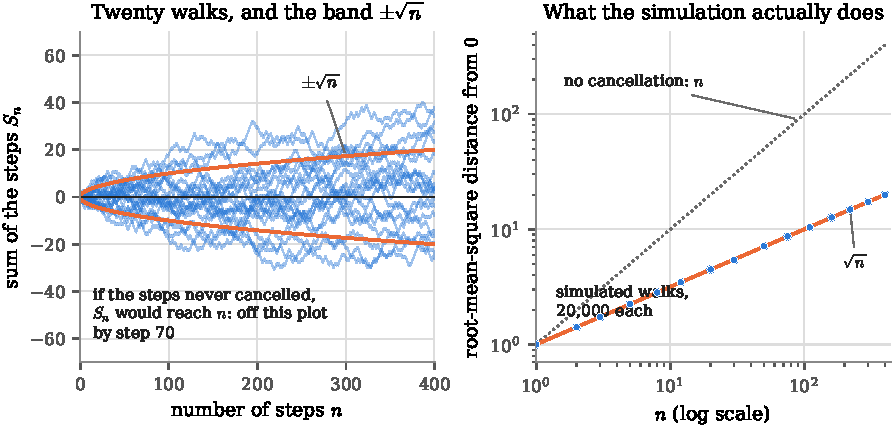
\includegraphics[width=\textwidth]{fig_why_root_n}
\caption{Where the $\sqrt{n}$ in every formula in this book comes from. Left: twenty running sums of steps of $+1$ and $-1$, each step equally likely, with the band $\pm\sqrt{n}$ drawn over them. If the steps never cancelled, the sum after $n$ steps would be $n$, which leaves the top of this figure by step $70$. Because they cancel, the sum stays inside a band that widens like $\sqrt{n}$. Right: the root-mean-square distance of the sum from zero, measured over $20{,}000$ simulated runs at each $n$, against $\sqrt{n}$ and against $n$ on logarithmic axes. The simulated points sit on $\sqrt{n}$, which is exact here: $\E[S_n^2] = n$, since each step has variance $1$ and the cross terms have expectation zero.}
\label{fig:whyrootn}
\end{figure}

\begin{sanitycheck}[The cost of precision]
Any time you produce a standard error, ask what it would take to halve it.
The answer is always four times the data, and it follows from the $\sqrt{n}$: to replace $\sigma/\sqrt{n}$ by $\sigma/(2\sqrt{n})$ you need $\sqrt{n}$ to double, so $n$ must quadruple.
If a calculation of yours implies that twice the data halves the error, you have divided by $n$ somewhere that should have been $\sqrt{n}$.
For the kiss experiment, the standard error at $n = 124$ is $0.043$; getting it to $0.02$ takes not $250$ couples but about $570$.
\end{sanitycheck}

Now, Chebyshev's inequality says that the probability that the distance of some r.v.\ from its mean is larger than some number, say $\epsilon$, is bounded above by the variance of the r.v.\ divided by $\epsilon^2$.
In the present context, the variance is $\sigma^2/n$, and so the upper bound is $\ds \frac{\sigma^2}{n \epsilon^2}$.
Formally, this is expressed as:
\[
\Pr(\abs{\bar{X}_n - \mu} \geq \epsilon) \leq \frac{\sigma^2}{n \epsilon^2}.
\]

The WLLN states that if $\epsilon$ is a fixed number and you take the limit of this probability as $n \to \infty$, then the limit converges to 0.
That is, the WLLN states that for any $\epsilon > 0$, as $n \to \infty$ you have:
\[
\Pr(\abs{\bar{X}_n - \mu} \geq \epsilon) = \Pr \left( \abs*{\frac{X_1 + \cdots + X_n}{n} - \mu} \geq \epsilon \right) \to 0.
\]

So the probability of falling far from the mean diminishes to zero as you draw more and more samples.

To make the interpretation of the WLLN more concrete, suppose again that you're conducting one long experiment, and during that experiment you draw $n$ i.i.d.\ r.v.s, $\Xton$, from the same parent distribution.
One way of thinking about the $X_i$ is that each one equals the true mean, $\mu$, plus some measurement noise, $U_i$, where $\E[U_i] = 0$ for all $i$ and the $U_i$ are independent.
You can then express these noisy measurements as $X_i = \mu + U_i$ for $i = 1, \ldots, n$.

So you've got a collection of noisy measurements and then you compute their average.
What the Weak Law of Large Numbers says is that the sample mean, $\bar{X}_n$, is unlikely to be far off from the true mean, $\mu$, of the parent distribution.
And by far off is meant at least $\epsilon$ distance away.
The sample mean is, thus, a good estimator of the true mean.

Here's the proof of the WLLN, which is easily demonstrated with Chebyshev's inequality.

\coreproof{Two lines: Chebyshev's inequality with $\var(\bar{X}_n) = \sigma^2/n$, then $n \to \infty$. This is the proof to know by heart.}
\begin{proof}
\leavevmode % Puts first item on next line
\begin{itemize}

\item Let $\epsilon$ be some positive real number.
Then by Chebyshev's inequality:
\[
\Pr(\abs{\bar{X}_n - \mu} \geq \epsilon) \leq \frac{\var(\bar{X}_n)}{\epsilon^2} = \frac{\sigma^2}{n \epsilon^2}.
\]

\item As $n \to \infty$, the right-hand side goes to 0, which implies $\Pr(\abs{\bar{X}_n - \mu} \geq \epsilon)$ goes to 0, too.
\end{itemize}
\end{proof}

\begin{worked}[the kiss experiment and Chebyshev]
In the kiss experiment $R_i \iid \Bern(p)$, so $\mu = p$ and $\sigma^2 = p(1-p)$.
How likely is it that the sample proportion misses $p$ by more than $0.084$ (about $10$ couples out of $124$)?
Chebyshev's inequality with $n = 124$, $\epsilon = 0.084$ and the worst case $p(1-p) \leq 1/4$ gives
\[
\Pr(\abs{\bar{R}_n - p} \geq 0.084) \leq \frac{p(1-p)}{n \epsilon^2} \leq \frac{0.25}{124 \times 0.084^2} \approx 0.29,
\]
and with $p(1-p)$ evaluated at $0.645$ the bound is $0.26$.
The bound is true but loose: the CLT (\cref{ch:clt}) says the probability is really about $0.05$.
Chebyshev's inequality is the right tool for proving that something converges, and the wrong tool for saying how fast.
\Cref{fig:bounds} in the next chapter shows all the bounds on the same axes.
\end{worked}

\begin{bridge}[consistency]
An estimator that converges in probability to the parameter it estimates is called \textit{consistent}.
The WLLN says the sample mean is a consistent estimator of the population mean, and the sample proportion is a consistent estimator of the population proportion.
In an introductory course you were told `with a bigger sample the estimate gets closer to the truth'; the WLLN is that sentence with every word defined.
Note what it does not say: it doesn't say $\bar{X}_n$ equals $\mu$ for any finite $n$, and it doesn't say how big $n$ must be for a given accuracy.
The CLT and Hoeffding's inequality, both in \cref{ch:clt}, handle the second question.
\end{bridge}

\section{What comes next}
\label{sec:lln-next}

The Law of Large Numbers says where $\bar{X}_n$ ends up: at $\mu$, with the variance $\sigma^2/n$ shrinking to nothing.
That's the left panel of \cref{fig:twoviews}, and it leaves the obvious question open.
If every density in that panel is on its way to becoming a spike, what does $\bar{X}_n$ look like \textit{along the way}?
The right panel already gave the answer in a picture: magnify the error by $\sqrt{n}$ and its shape settles down to a Gaussian, whatever the parent distribution.
Making that picture into a theorem needs the second mode of convergence, and it's the subject of the next chapter.

\section{Summary}
\label{sec:lln-summary}

\begin{itemize}[nosep]
\item A sequence of r.v.s is a sequence of functions on the sample space; one outcome fixes one ordinary sequence of numbers. No single index $N$ works for every outcome, so convergence has to be defined through probabilities.
\item `Asymptotic' means: for the $n$ at hand, replace the unknown sampling distribution by its limit, usually a Gaussian, and carry on; the theorem does not say how large $n$ must be.
\item $\bar{X}_n$ is a random variable, the theoretical sample mean; $\bar{x}_n$ is the number one sample produced. Every theorem is about the first. Its expectation is a second average, over all possible samples, of the first.
\item \textbf{Convergence in probability:} $X_n \convp X$ if $\Pr(\abs{X_n - X} \geq \epsilon) \to 0$ for every $\epsilon > 0$. The mass outside any band around the limit disappears.
\item \textbf{Shrinking-variance criterion:} $\E[T_n] \to \mu$ and $\var(T_n) \to 0$ imply $T_n \convp \mu$. This is Chebyshev's inequality, and it's how consistency is usually proved.
\item \textbf{Weak Law of Large Numbers:} $\bar{X}_n \convp \mu$ whenever the variance is finite because $\E[\bar{X}_n] = \mu$ and $\var(\bar{X}_n) = \sigma^2/n$. Estimators built from averages are consistent.
\item Chebyshev's bound $\sigma^2/(n\epsilon^2)$ is a guarantee at every $n$ but a loose one: $0.26$ in the kiss experiment where the truth is $0.05$.
\end{itemize}

\section{Exercises}
\label{sec:lln-exercises}

\begin{exercise}
Let $X_n \sim \Bern(1/n)$. (a) For $0 < \epsilon < 1$, what is $\Pr(\abs{X_n} > \epsilon)$? (b) Does $(X_n)$ converge in probability, and to what? (c) Does it converge in distribution? (d) What is $\lim_n \E[\cos(X_n)]$?
\end{exercise}
\begin{solution}
(a) $\Pr(\abs{X_n} > \epsilon) = \Pr(X_n = 1) = 1/n$. (b) Yes, to $0$, since $1/n \to 0$. (c) Yes, to $0$: convergence in probability implies convergence in distribution (\cref{prop:convp-implies-convd} in the next chapter), or directly, the CDF of $X_n$ is $1 - 1/n$ on $[0, 1)$ and $1$ from $1$ on, which converges to the CDF of the constant $0$ at every $x$ (at $x = 0$ too, here). (d) $\E[\cos X_n] = (1 - \frac1n)\cos 0 + \frac1n \cos 1 \to 1$; the next chapter's \cref{prop:convd-equiv} says this is no accident, since $\cos$ is continuous and bounded.
\end{solution}

\begin{exercise}
Let $\Xton \iid \Expo(\lambda)$, so $\E[X_1] = 1/\lambda$ and $\var(X_1) = 1/\lambda^2$. Use the shrinking-variance criterion to show that $\bar{X}_n \convp 1/\lambda$, and find the smallest $n$ for which Chebyshev's inequality guarantees $\Pr(\abs{\bar{X}_n - 1/\lambda} \geq 0.1/\lambda) \leq 0.05$.
\end{exercise}
\begin{solution}
$\E[\bar{X}_n] = 1/\lambda$ for every $n$ and $\var(\bar{X}_n) = 1/(n\lambda^2) \to 0$, so \cref{prop:shrinking-variance} applies. Chebyshev with $\epsilon = 0.1/\lambda$ gives $\Pr(\abs{\bar{X}_n - 1/\lambda} \geq 0.1/\lambda) \leq \frac{1/(n\lambda^2)}{0.01/\lambda^2} = \frac{100}{n}$, which is at most $0.05$ once $n \geq 2000$. The CLT of the next chapter, used as in its exercise 4, gives $n \approx 1.96^2/0.01 \approx 385$, which is the usual gap between a bound and the truth.
\end{solution}

\begin{exercise}
In the kiss model with $p = 0.645$, how many couples would Chebyshev's inequality require before $\Pr(\abs{\bar{R}_n - p} \geq 0.02) \leq 0.05$? Is the answer sensitive to $p$?
\end{exercise}
\begin{solution}
$\Pr(\abs{\bar{R}_n - p} \geq 0.02) \leq p(1-p)/(n \times 0.0004) \leq 0.05$ requires $n \geq p(1-p)/(0.00002) = 0.229/0.00002 \approx 11{,}450$. With the worst case $p(1-p) = 1/4$ the requirement is $12{,}500$; the dependence on $p$ is mild because $p(1-p)$ is flat near $1/2$.
\end{solution}
